% Options for packages loaded elsewhere
\PassOptionsToPackage{unicode}{hyperref}
\PassOptionsToPackage{hyphens}{url}
%
\documentclass[
]{book}
\usepackage{amsmath,amssymb}
\usepackage{lmodern}
\usepackage{iftex}
\ifPDFTeX
  \usepackage[T1]{fontenc}
  \usepackage[utf8]{inputenc}
  \usepackage{textcomp} % provide euro and other symbols
\else % if luatex or xetex
  \usepackage{unicode-math}
  \defaultfontfeatures{Scale=MatchLowercase}
  \defaultfontfeatures[\rmfamily]{Ligatures=TeX,Scale=1}
\fi
% Use upquote if available, for straight quotes in verbatim environments
\IfFileExists{upquote.sty}{\usepackage{upquote}}{}
\IfFileExists{microtype.sty}{% use microtype if available
  \usepackage[]{microtype}
  \UseMicrotypeSet[protrusion]{basicmath} % disable protrusion for tt fonts
}{}
\makeatletter
\@ifundefined{KOMAClassName}{% if non-KOMA class
  \IfFileExists{parskip.sty}{%
    \usepackage{parskip}
  }{% else
    \setlength{\parindent}{0pt}
    \setlength{\parskip}{6pt plus 2pt minus 1pt}}
}{% if KOMA class
  \KOMAoptions{parskip=half}}
\makeatother
\usepackage{xcolor}
\usepackage{color}
\usepackage{fancyvrb}
\newcommand{\VerbBar}{|}
\newcommand{\VERB}{\Verb[commandchars=\\\{\}]}
\DefineVerbatimEnvironment{Highlighting}{Verbatim}{commandchars=\\\{\}}
% Add ',fontsize=\small' for more characters per line
\usepackage{framed}
\definecolor{shadecolor}{RGB}{248,248,248}
\newenvironment{Shaded}{\begin{snugshade}}{\end{snugshade}}
\newcommand{\AlertTok}[1]{\textcolor[rgb]{0.94,0.16,0.16}{#1}}
\newcommand{\AnnotationTok}[1]{\textcolor[rgb]{0.56,0.35,0.01}{\textbf{\textit{#1}}}}
\newcommand{\AttributeTok}[1]{\textcolor[rgb]{0.77,0.63,0.00}{#1}}
\newcommand{\BaseNTok}[1]{\textcolor[rgb]{0.00,0.00,0.81}{#1}}
\newcommand{\BuiltInTok}[1]{#1}
\newcommand{\CharTok}[1]{\textcolor[rgb]{0.31,0.60,0.02}{#1}}
\newcommand{\CommentTok}[1]{\textcolor[rgb]{0.56,0.35,0.01}{\textit{#1}}}
\newcommand{\CommentVarTok}[1]{\textcolor[rgb]{0.56,0.35,0.01}{\textbf{\textit{#1}}}}
\newcommand{\ConstantTok}[1]{\textcolor[rgb]{0.00,0.00,0.00}{#1}}
\newcommand{\ControlFlowTok}[1]{\textcolor[rgb]{0.13,0.29,0.53}{\textbf{#1}}}
\newcommand{\DataTypeTok}[1]{\textcolor[rgb]{0.13,0.29,0.53}{#1}}
\newcommand{\DecValTok}[1]{\textcolor[rgb]{0.00,0.00,0.81}{#1}}
\newcommand{\DocumentationTok}[1]{\textcolor[rgb]{0.56,0.35,0.01}{\textbf{\textit{#1}}}}
\newcommand{\ErrorTok}[1]{\textcolor[rgb]{0.64,0.00,0.00}{\textbf{#1}}}
\newcommand{\ExtensionTok}[1]{#1}
\newcommand{\FloatTok}[1]{\textcolor[rgb]{0.00,0.00,0.81}{#1}}
\newcommand{\FunctionTok}[1]{\textcolor[rgb]{0.00,0.00,0.00}{#1}}
\newcommand{\ImportTok}[1]{#1}
\newcommand{\InformationTok}[1]{\textcolor[rgb]{0.56,0.35,0.01}{\textbf{\textit{#1}}}}
\newcommand{\KeywordTok}[1]{\textcolor[rgb]{0.13,0.29,0.53}{\textbf{#1}}}
\newcommand{\NormalTok}[1]{#1}
\newcommand{\OperatorTok}[1]{\textcolor[rgb]{0.81,0.36,0.00}{\textbf{#1}}}
\newcommand{\OtherTok}[1]{\textcolor[rgb]{0.56,0.35,0.01}{#1}}
\newcommand{\PreprocessorTok}[1]{\textcolor[rgb]{0.56,0.35,0.01}{\textit{#1}}}
\newcommand{\RegionMarkerTok}[1]{#1}
\newcommand{\SpecialCharTok}[1]{\textcolor[rgb]{0.00,0.00,0.00}{#1}}
\newcommand{\SpecialStringTok}[1]{\textcolor[rgb]{0.31,0.60,0.02}{#1}}
\newcommand{\StringTok}[1]{\textcolor[rgb]{0.31,0.60,0.02}{#1}}
\newcommand{\VariableTok}[1]{\textcolor[rgb]{0.00,0.00,0.00}{#1}}
\newcommand{\VerbatimStringTok}[1]{\textcolor[rgb]{0.31,0.60,0.02}{#1}}
\newcommand{\WarningTok}[1]{\textcolor[rgb]{0.56,0.35,0.01}{\textbf{\textit{#1}}}}
\usepackage{longtable,booktabs,array}
\usepackage{calc} % for calculating minipage widths
% Correct order of tables after \paragraph or \subparagraph
\usepackage{etoolbox}
\makeatletter
\patchcmd\longtable{\par}{\if@noskipsec\mbox{}\fi\par}{}{}
\makeatother
% Allow footnotes in longtable head/foot
\IfFileExists{footnotehyper.sty}{\usepackage{footnotehyper}}{\usepackage{footnote}}
\makesavenoteenv{longtable}
\usepackage{graphicx}
\makeatletter
\def\maxwidth{\ifdim\Gin@nat@width>\linewidth\linewidth\else\Gin@nat@width\fi}
\def\maxheight{\ifdim\Gin@nat@height>\textheight\textheight\else\Gin@nat@height\fi}
\makeatother
% Scale images if necessary, so that they will not overflow the page
% margins by default, and it is still possible to overwrite the defaults
% using explicit options in \includegraphics[width, height, ...]{}
\setkeys{Gin}{width=\maxwidth,height=\maxheight,keepaspectratio}
% Set default figure placement to htbp
\makeatletter
\def\fps@figure{htbp}
\makeatother
\setlength{\emergencystretch}{3em} % prevent overfull lines
\providecommand{\tightlist}{%
  \setlength{\itemsep}{0pt}\setlength{\parskip}{0pt}}
\setcounter{secnumdepth}{5}
\usepackage{booktabs}
\ifLuaTeX
  \usepackage{selnolig}  % disable illegal ligatures
\fi
\usepackage[]{natbib}
\bibliographystyle{plainnat}
\IfFileExists{bookmark.sty}{\usepackage{bookmark}}{\usepackage{hyperref}}
\IfFileExists{xurl.sty}{\usepackage{xurl}}{} % add URL line breaks if available
\urlstyle{same} % disable monospaced font for URLs
\hypersetup{
  pdftitle={A Minimal Book for Metamazon},
  pdfauthor={Marion Boisseaux},
  hidelinks,
  pdfcreator={LaTeX via pandoc}}

\title{A Minimal Book for Metamazon}
\author{Marion Boisseaux}
\date{2024-09-03}

\begin{document}
\maketitle

{
\setcounter{tocdepth}{1}
\tableofcontents
}
\hypertarget{about}{%
\chapter{About}\label{about}}

This is a \emph{sample} book for the \textbf{Metamazon} IRD (Institut de Recherche pour le développement) project.

\textbf{Nicolas Hubert} (UMR ISEM), ictiólogo y genetista, inicia su misión en Perú para desarrollar el Observatorio de Biodiversidad de la Amazonía Peruana (OBAP) con \textbf{Carmen García-Dávila}, presidenta ejecutiva del IIAP (Instituto de Investigaciones de la Amazonía Peruana).

Este programa de investigación irá acompañado de un proyecto de formación de \emph{tres} años en la potente técnica de metabarcoding del ADN ambiental (ADNa), que permite obtener información sobre la biodiversidad de un ecosistema a partir de muestras de agua, suelo o aire. El curso abarcará técnicas de muestreo, extracción de ADNa, amplificación y métodos de análisis de datos.

\hypertarget{year-2024}{%
\chapter{Year 2024}\label{year-2024}}

Here is the program for the first year of the project.

\hypertarget{semana-de-formaciuxf3n-virtual-metamazon-del-1-al-5-de-julio-2024}{%
\section{Semana de formación virtual METAMAZON del 1 al 5 de julio 2024}\label{semana-de-formaciuxf3n-virtual-metamazon-del-1-al-5-de-julio-2024}}

La próxima semana tendrá lugar nuestra sesión de formación virtual. En total, 12 formadores intervendrán durante la semana para abordar diferentes aspectos del uso de códigos de barras de ADN desde la presentación general del enfoque hasta reconstrucción filogenética y genética de poblaciones para la delimitación de especies y el uso de bases de datos internacionales de códigos de barra.

Todos los cursos serán accesibles online desde este único enlace durante toda la semana: \_\url{https://umontpellier-fr.zoom.us/j/93830263869_}

La capacitación se realizará todos los días de lunes a viernes de las \emph{9:00} hasta las \emph{13:00} (GMT-5:00 - Lima) y incluirá una parte de cursos cuál terminará con una sesión de preguntas a las que responderán los profesores del día.

El programa detallado de la semana se encuentra aqui:

\begin{itemize}
\tightlist
\item
  \href{programa/Programa_july2024.pdf}{Programa July 2024}
\end{itemize}

\hypertarget{taller-iquitos}{%
\section{Taller Iquitos}\label{taller-iquitos}}

Estamos a menos de 7 días de nuestro taller en Iquitos. Para que se pueden preparar lo mejor possible, y que su llegada se pase bien, los mandemos el programa del taller que incluye:
- el programa actualizado de la semana
- informaciones prácticas sobre la organización del taller
- anuario de los participantes

\begin{itemize}
\tightlist
\item
  \href{programa/Programa_METAMAZON_Agosto_2024.pdf}{Programa Agosto 2024}
\end{itemize}

\hypertarget{script-2024}{%
\section{Script 2024}\label{script-2024}}

\hypertarget{packages}{%
\section*{Packages}\label{packages}}
\addcontentsline{toc}{section}{Packages}

\hypertarget{libraries}{%
\section*{Libraries}\label{libraries}}
\addcontentsline{toc}{section}{Libraries}

\begin{Shaded}
\begin{Highlighting}[]
\FunctionTok{library}\NormalTok{(devtools)}
\FunctionTok{library}\NormalTok{(rentrez)}
\FunctionTok{library}\NormalTok{(phylotools)}
\FunctionTok{library}\NormalTok{(readr)}
\FunctionTok{library}\NormalTok{(seqRFLP)}
\FunctionTok{library}\NormalTok{(dplyr)}
\FunctionTok{library}\NormalTok{(ape)}
\FunctionTok{library}\NormalTok{(BarcodingR)}
\FunctionTok{library}\NormalTok{(splits)}
\FunctionTok{library}\NormalTok{(bold)}
\FunctionTok{library}\NormalTok{(splits)}
\end{Highlighting}
\end{Shaded}

\hypertarget{descargar-desde-genbank}{%
\section*{Descargar desde GenBank}\label{descargar-desde-genbank}}
\addcontentsline{toc}{section}{Descargar desde GenBank}

\hypertarget{peru}{%
\subsection*{Peru}\label{peru}}
\addcontentsline{toc}{subsection}{Peru}

To obtain an API Key through your NCBI account, follow these steps:

\begin{itemize}
\tightlist
\item
  Sign in to your NCBI account.
\item
  Once signed in, access your account's settings by clicking on your user name which is displayed in the top right corner of any NCBI page.
\item
  Account settings
\item
  Scroll down the page to the section entitled API Key Management.
\item
  Click the Create an API Key button, which will generate a key (unique sequence of characters) displayed in the API Key Management box.
\end{itemize}

\hypertarget{brasil}{%
\section*{Brasil}\label{brasil}}
\addcontentsline{toc}{section}{Brasil}

\hypertarget{bold}{%
\section*{BOLD}\label{bold}}
\addcontentsline{toc}{section}{BOLD}

\hypertarget{how-to-do-trees-using-r}{%
\section*{How to do trees using R ?}\label{how-to-do-trees-using-r}}
\addcontentsline{toc}{section}{How to do trees using R ?}

\begin{Shaded}
\begin{Highlighting}[]
\NormalTok{tree }\OtherTok{\textless{}{-}} \FunctionTok{read.tree}\NormalTok{(}\StringTok{"Data/MCT\_barbo\_gmyc.nwk"}\NormalTok{)}

\NormalTok{gmyc\_single }\OtherTok{\textless{}{-}} \FunctionTok{gmyc}\NormalTok{(tree, }\AttributeTok{method =} \StringTok{"single"}\NormalTok{) }\CommentTok{\#Optimizes genetic clusters using the generalized mixed yule coalescent.}
\end{Highlighting}
\end{Shaded}

\begin{verbatim}
## node  T   loglik
## 2 -3.055273 390.5014 
## 3 -2.620138 392.2448 
## 4 -2.218061 393.8758 
## 5 -1.142561 396.8952 
## 6 -0.6267099 398.1031 
## 7 -0.5476014 397.0213 
## 8 -0.5382909 395.995 
## 9 -0.4433933 395.7144 
## 10 -0.4305619 395.1131 
## 11 -0.4065495 394.9445 
## 12 -0.3851693 394.8939 
## 13 -0.381523 394.6614 
## 14 -0.349054 394.5592 
## 15 -0.3310504 394.3957 
## 16 -0.329897 394.2457 
## 17 -0.3070474 393.8311 
## 18 -0.2845661 393.7635 
## 19 -0.2681086 393.6039 
## 20 -0.2679646 393.3894 
## 21 -0.2537394 393.4403 
## 22 -0.2521766 393.215 
## 23 -0.2419285 393.0034 
## 24 -0.2374474 392.887 
## 25 -0.2338045 392.6641 
## 26 -0.2191677 392.4317 
## 27 -0.2186199 391.4239 
## 28 -0.2167877 391.3184 
## 29 -0.2163702 391.0074 
## 30 -0.2141133 390.8574 
## 31 -0.2054208 390.2979 
## 32 -0.1958052 390.047 
## 33 -0.1891496 389.7879 
## 34 -0.1825583 389.0644 
## 35 -0.1783501 388.8971 
## 36 -0.1753595 388.1967 
## 37 -0.1713631 389.701 
## 38 -0.1711421 389.7677 
## 39 -0.1623105 389.3054 
## 40 -0.1586686 389.1617 
## 41 -0.1575343 388.969 
## 42 -0.1574083 388.8982 
## 43 -0.1425217 389.0109 
## 44 -0.1422395 389.1973 
## 45 -0.1370439 389.1257 
## 46 -0.133169 389.2907 
## 47 -0.1196028 389.4891 
## 48 -0.1143404 389.8565 
## 49 -0.1015881 389.6223 
## 50 -0.0966579 389.4921 
## 51 -0.08908788 389.6775 
## 52 -0.08486527 389.6584 
## 53 -0.07848787 389.6604 
## 54 -0.07532674 389.6093 
## 55 -0.07005008 389.5649 
## 56 -0.06968558 389.0122 
## 57 -0.06491394 388.6848 
## 58 -0.06149535 388.7406 
## 59 -0.0601955 388.7775 
## 60 -0.05958394 388.6472 
## 61 -0.05681971 388.5208 
## 62 -0.05550206 388.1066 
## 63 -0.05523072 388.0301 
## 64 -0.05486178 387.9217 
## 65 -0.05426426 387.8233 
## 66 -0.05360742 387.4405 
## 67 -0.04444144 387.3129 
## 68 -0.0406332 387.0265 
## 69 -0.04052827 386.8101 
## 70 -0.03831684 386.59 
## 71 -0.0359657 386.5652 
## 72 -0.03357435 386.5556 
## 73 -0.03269212 386.5643 
## 74 -0.03261033 386.5833 
## 75 -0.03154326 386.6061 
## 76 -0.03079578 386.64 
## 77 -0.03001186 386.7042 
## 78 -0.02922072 386.779 
## 79 -0.02780451 386.8652 
## 80 -0.02711191 386.9724 
## 81 -0.02681365 387.0922 
## 82 -0.02673203 387.2192 
## 83 -0.02669239 387.35 
## 84 -0.02452315 387.4832 
## 85 -0.02400853 387.6568 
## 86 -0.02349517 387.8446 
## 87 -0.02318273 388.0476 
## 88 -0.02290598 388.2626 
## 89 -0.02283918 388.4896 
## 90 -0.02225487 388.7246 
## 91 -0.02166405 388.98 
## 92 -0.02085182 389.258 
## 93 -0.01963487 389.5659 
## 94 -0.0190678 389.9174 
## 95 -0.01894042 390.2993 
## 
## Tue Sep  3 21:19:00 2024
## finish.
\end{verbatim}

\begin{Shaded}
\begin{Highlighting}[]
\NormalTok{splits}\SpecialCharTok{::}\FunctionTok{summary.gmyc}\NormalTok{(gmyc\_single) }\CommentTok{\# summary statistics of the results}
\end{Highlighting}
\end{Shaded}

\begin{verbatim}
## Result of GMYC species delimitation
## 
##  method: single
##  likelihood of null model:   391.276
##  maximum likelihood of GMYC model:   398.1031
##  likelihood ratio:   13.65415
##  result of LR test:  0.001084025**
## 
##  number of ML clusters:  3
##  confidence interval:    3-4
## 
##  number of ML entities:  6
##  confidence interval:    5-7
## 
##  threshold time: -0.6267099
\end{verbatim}

\begin{Shaded}
\begin{Highlighting}[]
\FunctionTok{plot.gmyc}\NormalTok{(gmyc\_single) }\CommentTok{\# lineage through time with inferred threshold}
\end{Highlighting}
\end{Shaded}

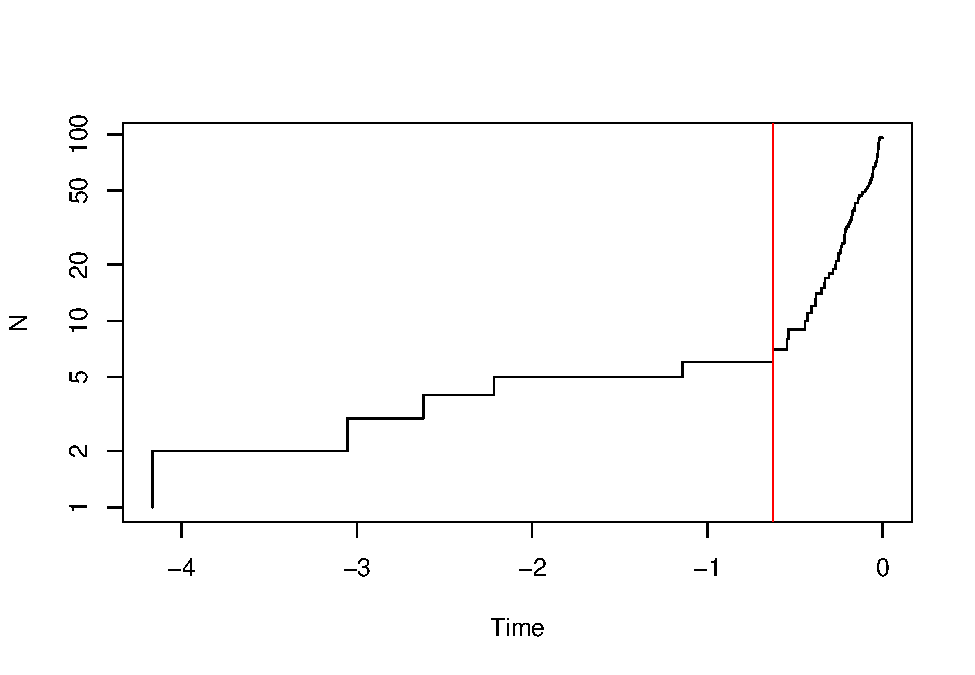
\includegraphics{_main_files/figure-latex/unnamed-chunk-4-1.pdf} 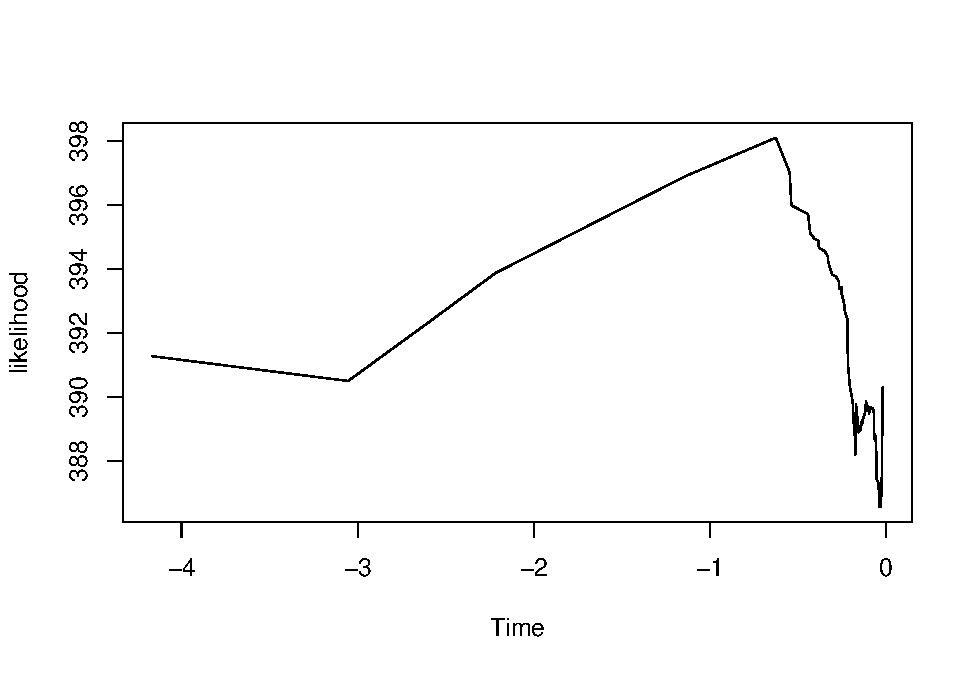
\includegraphics{_main_files/figure-latex/unnamed-chunk-4-2.pdf} 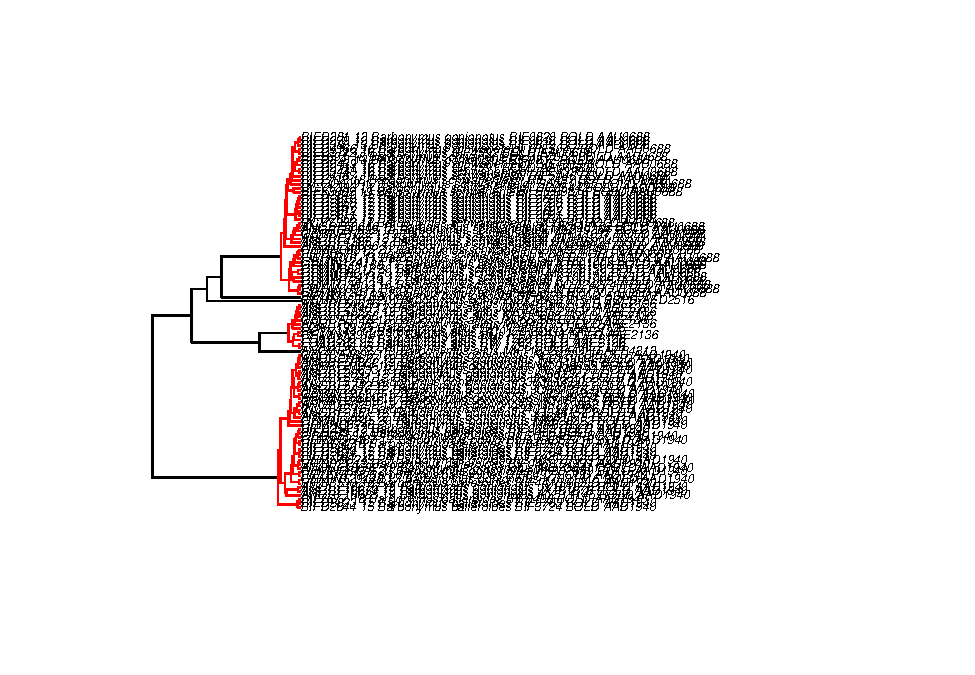
\includegraphics{_main_files/figure-latex/unnamed-chunk-4-3.pdf}

\begin{Shaded}
\begin{Highlighting}[]
\NormalTok{MOTU\_list}\OtherTok{\textless{}{-}}\FunctionTok{spec.list}\NormalTok{(gmyc\_single) }\CommentTok{\# list of MOTUs and individuals}
\FunctionTok{write.csv}\NormalTok{(MOTU\_list, }\AttributeTok{file =} \StringTok{"Data/MOTU\_gmyc\_single.csv"}\NormalTok{) }\CommentTok{\# export the list in csv format}
\NormalTok{support }\OtherTok{\textless{}{-}} \FunctionTok{gmyc.support}\NormalTok{(gmyc\_single) }\CommentTok{\# estimate support}
\FunctionTok{is.na}\NormalTok{(support[support }\SpecialCharTok{==} \DecValTok{0}\NormalTok{]) }\OtherTok{\textless{}{-}} \ConstantTok{TRUE} \CommentTok{\# select nodes}
\FunctionTok{plot}\NormalTok{(tree, }\AttributeTok{cex =} \FloatTok{0.4}\NormalTok{, }\AttributeTok{no.margin =} \ConstantTok{TRUE}\NormalTok{) }\CommentTok{\# plot tree}
\FunctionTok{nodelabels}\NormalTok{(}\FunctionTok{round}\NormalTok{(support, }\DecValTok{2}\NormalTok{), }\AttributeTok{cex =} \FloatTok{0.9}\NormalTok{) }\CommentTok{\# plot support on tree}
\end{Highlighting}
\end{Shaded}

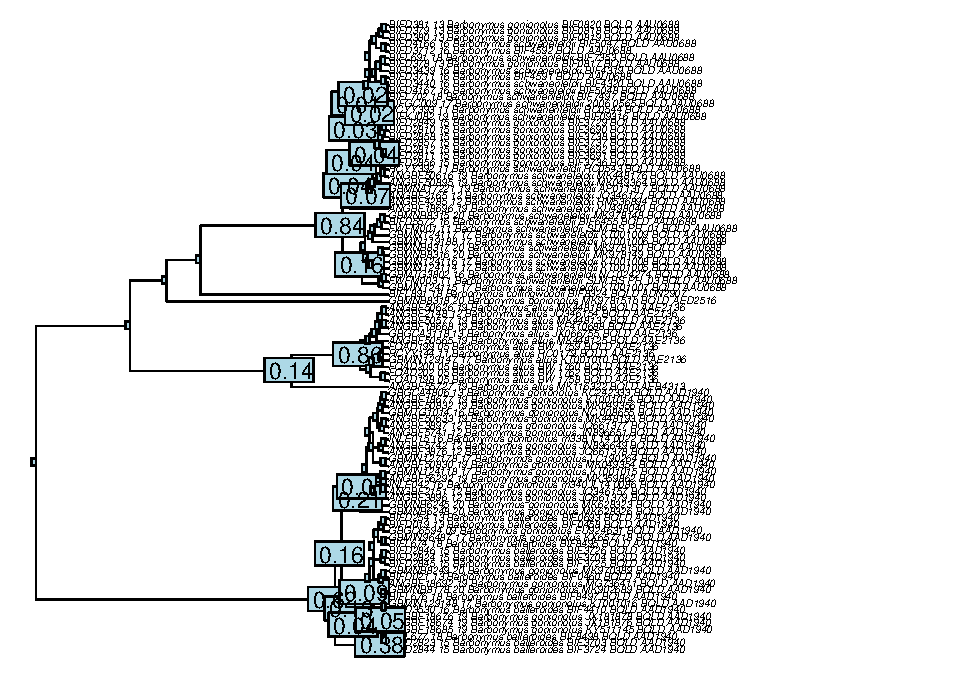
\includegraphics{_main_files/figure-latex/unnamed-chunk-4-4.pdf}

\hypertarget{asignaciuxf3n-de-secuencias-desconocidas-a-una-libreruxeda-de-referencia-con-otros-muxe9todos-paquete-r-barcodingr}{%
\section*{Asignación de secuencias desconocidas a una librería de referencia con otros métodos (paquete R BarcodingR)}\label{asignaciuxf3n-de-secuencias-desconocidas-a-una-libreruxeda-de-referencia-con-otros-muxe9todos-paquete-r-barcodingr}}
\addcontentsline{toc}{section}{Asignación de secuencias desconocidas a una librería de referencia con otros métodos (paquete R BarcodingR)}

\begin{Shaded}
\begin{Highlighting}[]
\NormalTok{REF }\OtherTok{\textless{}{-}} \FunctionTok{read.dna}\NormalTok{(}\StringTok{"Data/Barbonymus\_REF.fasta"}\NormalTok{, }\AttributeTok{format =} \StringTok{"fasta"}\NormalTok{)}
\NormalTok{ID }\OtherTok{\textless{}{-}} \FunctionTok{read.dna}\NormalTok{(}\StringTok{"Data/Barbonymus\_ID.fasta"}\NormalTok{, }\AttributeTok{format =} \StringTok{"fasta"}\NormalTok{)}

\CommentTok{\#3 diferentes metodos para obtener la identification y la probabilidad}
\CommentTok{\#comme des BLAST en local avec différentes méthodes, car on donne des FASTA}
\NormalTok{fuzzyId}\OtherTok{\textless{}{-}}\FunctionTok{barcoding.spe.identify}\NormalTok{(REF, ID, }\AttributeTok{method =} \StringTok{"fuzzyId"}\NormalTok{)}
\NormalTok{Bayesian}\OtherTok{\textless{}{-}}\FunctionTok{barcoding.spe.identify}\NormalTok{(REF, ID, }\AttributeTok{method =} \StringTok{"Bayesian"}\NormalTok{)}
\NormalTok{BP}\OtherTok{\textless{}{-}}\FunctionTok{barcoding.spe.identify}\NormalTok{(REF, ID, }\AttributeTok{method =} \StringTok{"bpNewTraining"}\NormalTok{)}
\end{Highlighting}
\end{Shaded}

\begin{verbatim}
## # weights:  390
## initial  value 14.469968 
## iter  10 value 3.882162
## iter  20 value 0.301800
## iter  30 value 0.184916
## iter  40 value 0.155602
## iter  50 value 0.127458
## iter  60 value 0.104251
## iter  70 value 0.095517
## iter  80 value 0.090452
## iter  90 value 0.084658
## iter 100 value 0.080322
## iter 110 value 0.078020
## iter 120 value 0.074008
## iter 130 value 0.071581
## iter 140 value 0.069977
## iter 150 value 0.068903
## iter 160 value 0.067612
## iter 170 value 0.065193
## iter 180 value 0.064245
## iter 190 value 0.063400
## iter 200 value 0.063071
## iter 210 value 0.063009
## iter 220 value 0.062951
## iter 230 value 0.062922
## iter 240 value 0.062894
## iter 250 value 0.062836
## iter 260 value 0.062590
## iter 270 value 0.062537
## iter 280 value 0.062085
## iter 290 value 0.061787
## iter 300 value 0.061700
## iter 310 value 0.061604
## iter 320 value 0.061585
## iter 330 value 0.061581
## iter 340 value 0.061577
## iter 350 value 0.061571
## iter 360 value 0.061501
## iter 370 value 0.061490
## iter 380 value 0.061414
## iter 390 value 0.061400
## iter 400 value 0.061398
## final  value 0.061397 
## converged
\end{verbatim}

\hypertarget{articulos}{%
\section{Articulos}\label{articulos}}

\begin{itemize}
\item
  \textbf{Artículo 1} Hubert, Nicolas, et al.~``Identifying Canadian freshwater fishes through DNA barcodes.'' \emph{PLoS one} 3.6 (2008): e2490. \href{articulos/Articulo_1-Hubert_et_al_2008.pdf}{Articulo 1}
\item
  \textbf{Artículo 2} CBOL Plant Working Group 1, et al.~``A DNA barcode for land plants.'' \emph{Proceedings of the National Academy of Sciences} 106.31 (2009): 12794-12797. \href{articulos/Articulo_2-Hollingsworth_et_al_2009.pdf}{Articulo 2}
\item
  \textbf{Artículo 3} Truong, Camille, et al.~``Ectomycorrhizal fungi and soil enzymes exhibit contrasting patterns along elevation gradients in southern Patagonia.'' \emph{New Phytologist} 222.4 (2019): 1936-1950. \href{articulos/Articulo_3_Truong-knowfungi-2017.pdf}{Articulo 3}
\end{itemize}

\href{articulos/articulo3_90004204-sup-0001-SupInfo.pdf}{Supplementary Articulo 3}

\begin{itemize}
\item
  \textbf{Artículo 4} Blair, Christopher, and Robert W. Bryson Jr.~``Cryptic diversity and discordance in single-locus species delimitation methods within horned lizards (Phrynosomatidae: Phrynosoma).'' \emph{Molecular Ecology Resources} 17.6 (2017): 1168-1182. \href{articulos/Articulo_4-Blair_et_al_2017.pdf}{Articulo 4}
\item
  \textbf{Artículo 5} Puillandre, Nicolas, Sophie Brouillet, and Guillaume Achaz. ``ASAP: assemble species by automatic partitioning.'' \emph{Molecular Ecology Resources} 21.2 (2021): 609-620. \href{articulos/Articulo_5-Puillandre_et_al_2020.pdf}{Articulo 5}
\item
  \textbf{Artículo 6} Arida, Evy, et al.~``Exploring the vertebrate fauna of the Bird's Head Peninsula (Indonesia, West Papua) through DNA barcodes.'' \emph{Molecular Ecology Resources} 21.7 (2021): 2369-2387. \href{articulos/Articulo_6-Arida_et_al_2021.pdf}{Articulo 6}
\end{itemize}

\hypertarget{presentaciones-de-los-participantes}{%
\section{Presentaciones de los participantes}\label{presentaciones-de-los-participantes}}

Cada participante prepara un powerpoint para presentarse y presentar su experiencia de trabajo de laboratorio, protocolos de extracción y técnicas de secuenciación, presentación de sus temas de investigación y
modelos biológicos.

\href{presentaciones_participantes/MBoisseaux.pdf}{Marion Boisseaux}

\hypertarget{reserva-nacional-allpahuayo-mishana}{%
\section{Reserva nacional Allpahuayo Mishana}\label{reserva-nacional-allpahuayo-mishana}}

! \href{photos/20240829_070712.jpg}{Reserva nacional Allpahuayo Mishana}

Recogida de muestras, técnica de muestreo y conservación, presentación de procedimientos de adquisición de datos de campo en un contexto de código de barras de ADN, gestión de una colección de trabajo.

Presentación \textbf{Nicolas Hubert} sobre los procedimientos para códigos de barra

Presentación Nora Scarcelli y Mélanie Roy sobre el muestreo de plantas y
hongos, gestión de colección y procedimientos para códigos de barra

Presentación Guido sobre muestreo larva de peces

Presentación Dario Acha sobre colecta de muestras de microorganismos

\hypertarget{cross}{%
\chapter{Cross-references}\label{cross}}

Cross-references make it easier for your readers to find and link to elements in your book.

\hypertarget{chapters-and-sub-chapters}{%
\section{Chapters and sub-chapters}\label{chapters-and-sub-chapters}}

There are two steps to cross-reference any heading:

\begin{enumerate}
\def\labelenumi{\arabic{enumi}.}
\tightlist
\item
  Label the heading: \texttt{\#\ Hello\ world\ \{\#nice-label\}}.

  \begin{itemize}
  \tightlist
  \item
    Leave the label off if you like the automated heading generated based on your heading title: for example, \texttt{\#\ Hello\ world} = \texttt{\#\ Hello\ world\ \{\#hello-world\}}.
  \item
    To label an un-numbered heading, use: \texttt{\#\ Hello\ world\ \{-\#nice-label\}} or \texttt{\{\#\ Hello\ world\ .unnumbered\}}.
  \end{itemize}
\item
  Next, reference the labeled heading anywhere in the text using \texttt{\textbackslash{}@ref(nice-label)}; for example, please see Chapter \ref{cross}.

  \begin{itemize}
  \tightlist
  \item
    If you prefer text as the link instead of a numbered reference use: \protect\hyperlink{cross}{any text you want can go here}.
  \end{itemize}
\end{enumerate}

\hypertarget{captioned-figures-and-tables}{%
\section{Captioned figures and tables}\label{captioned-figures-and-tables}}

Figures and tables \emph{with captions} can also be cross-referenced from elsewhere in your book using \texttt{\textbackslash{}@ref(fig:chunk-label)} and \texttt{\textbackslash{}@ref(tab:chunk-label)}, respectively.

See Figure \ref{fig:nice-fig}.

\begin{Shaded}
\begin{Highlighting}[]
\FunctionTok{par}\NormalTok{(}\AttributeTok{mar =} \FunctionTok{c}\NormalTok{(}\DecValTok{4}\NormalTok{, }\DecValTok{4}\NormalTok{, .}\DecValTok{1}\NormalTok{, .}\DecValTok{1}\NormalTok{))}
\FunctionTok{plot}\NormalTok{(pressure, }\AttributeTok{type =} \StringTok{\textquotesingle{}b\textquotesingle{}}\NormalTok{, }\AttributeTok{pch =} \DecValTok{19}\NormalTok{)}
\end{Highlighting}
\end{Shaded}

\begin{figure}

{\centering 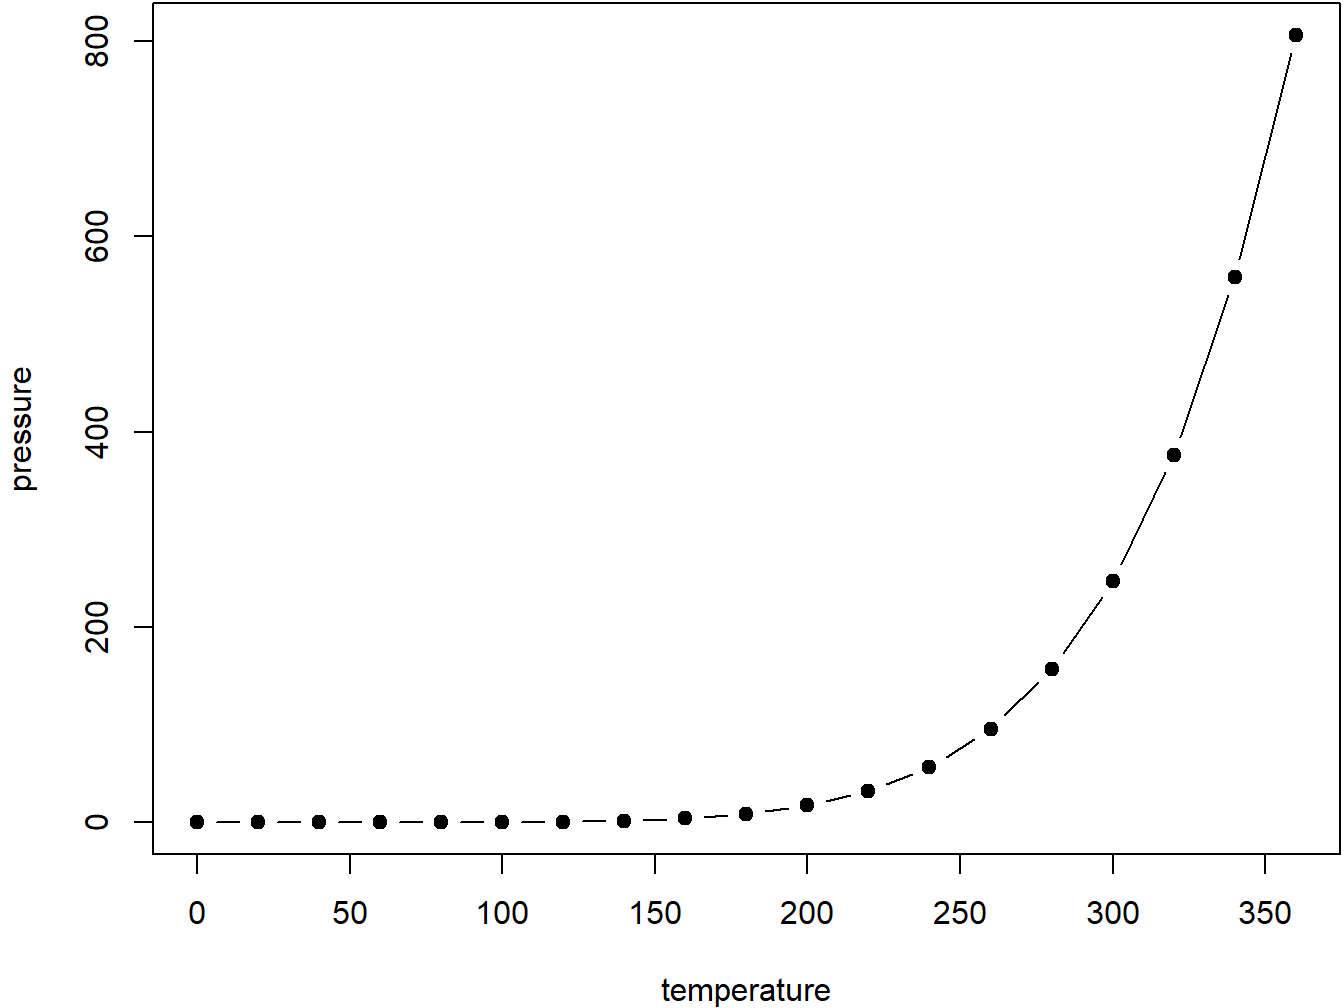
\includegraphics[width=0.8\linewidth]{_main_files/figure-latex/nice-fig-1} 

}

\caption{Here is a nice figure!}\label{fig:nice-fig}
\end{figure}

Don't miss Table \ref{tab:nice-tab}.

\begin{Shaded}
\begin{Highlighting}[]
\NormalTok{knitr}\SpecialCharTok{::}\FunctionTok{kable}\NormalTok{(}
  \FunctionTok{head}\NormalTok{(pressure, }\DecValTok{10}\NormalTok{), }\AttributeTok{caption =} \StringTok{\textquotesingle{}Here is a nice table!\textquotesingle{}}\NormalTok{,}
  \AttributeTok{booktabs =} \ConstantTok{TRUE}
\NormalTok{)}
\end{Highlighting}
\end{Shaded}

\begin{table}

\caption{\label{tab:nice-tab}Here is a nice table!}
\centering
\begin{tabular}[t]{rr}
\toprule
temperature & pressure\\
\midrule
0 & 0.0002\\
20 & 0.0012\\
40 & 0.0060\\
60 & 0.0300\\
80 & 0.0900\\
\addlinespace
100 & 0.2700\\
120 & 0.7500\\
140 & 1.8500\\
160 & 4.2000\\
180 & 8.8000\\
\bottomrule
\end{tabular}
\end{table}

  \bibliography{book.bib,packages.bib}

\end{document}
